\documentclass[12pt]{article}
\usepackage[utf8]{inputenc}
\usepackage[margin=1in]{geometry}
\usepackage[spanish]{babel}\decimalpoint
\usepackage{setspace}\onehalfspacing
\usepackage{parskip} %Espacio entre parrafos.
\usepackage{graphicx} %Para usar \includegraphics[]{}
\usepackage{amssymb} %Para usar el simbolo del conj. de los Reales.%
\usepackage{amsmath} % Para usar columnas vectoriales.
\usepackage{multirow}
\usepackage{hyperref} %Siempre debe ser el ultimo paquete.


%\setlength{\parindent}{0pt} %Texto justificado.
\setcounter{tocdepth}{2} %Que no incluya subsubsections en el índice.

%================================

\title{Clase 18: Introducción a la Integral Definida.}
\author{MIT 18.01: Single Variable Calculus.}
\date{}

\begin{document}
\maketitle

\begin{abstract}
{\noindent
En esta ocasión introduciremos a la \textbf{Integral Definida}, la cual es similar a la integral indefinida (o infinitesimal) en cuanto a su notación, pero se diferencia en que corresponde a \textbf{un número} y no a una familia de funciones. En particular, nos entrega el área bajo la curva de una función y se obtiene a partir del \textbf{límite al infinito de la Suma de Riemann}. Por ello también es interpretada como una \textbf{suma acumulada}.
}
\end{abstract}


\section{La Integral Definida.}

Cuando nos enfrentamos al \textbf{problema geométrico} de conocer el área bajo la curva de una función, desde el Cálculo lo hacemos por medio de la \textbf{Integral Definida}, la cual denotamos como:
\[
  \int_{a}^{b} f(x)dx
\]
Su notación es similar a la integral indefinida, pero se incluyen los límites inferior $a$ y superior $b$ que delimitan el área a calcular de la curva, la cual está dada por su integrando $f(x)$. También se diferencia de la indefinida en que nos entrega \textbf{un número} y no una familia de funciones. No obstante, en la siguiente clase veremos que ambas se relacionan.

La integral definida es útil cuando queremos obtener el área bajo una curva que no es lineal, como la que vemos a continuación.

\begin{figure}[hbt!]
\centering
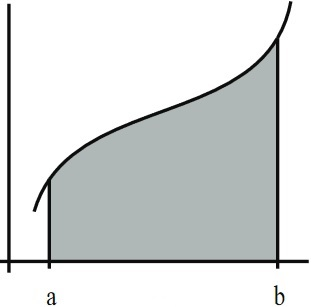
\includegraphics[scale=0.5]{img/area-under-curve.jpg}
\end{figure}

\subsection{Calculando el área bajo una curva y la Suma de Riemann.}

Para calcular el área de una curva no lineal, seguimos los siguientes pasos:

\textbf{1. Dividir el área en rectángulos de igual base.} \quad Si bien el área se puede dividir usando distintas figuras geométricas, la más habitual es el rectángulo, pero serán hipotéticos porque algunos cubrirán más (exceso) o menos (déficit) de lo necesario.

\begin{figure}[hbt!]
\centering
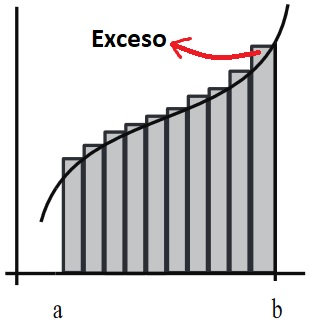
\includegraphics[scale=0.5]{img/area-under-curve-2.jpg}
\end{figure}

Por otra parte, los rectángulos que usamos son todos de \textbf{igual base}.

\textbf{2. Sumar las áreas de los rectángulos.} \quad Al dividir el área en rectángulos, se forma una región cuya área es la suma de las áreas de estas figuras, conocida como la \textbf{Suma de Riemann}. En este punto, el exceso o déficit estará incluido en aquel valor, por lo que aún no tendremos el exacto (o más cercano) al de interés.

\textbf{3. Tomar el límite al infinito de la suma.} \quad Para que el error de la suma de Riemann sea cero, tenemos que dividir el área en una gran cantidad de rectángulos, tal como lo vemos a continuación, donde $n$ es la cantidad de particiones del área.

\begin{figure}[hbt!]
\centering
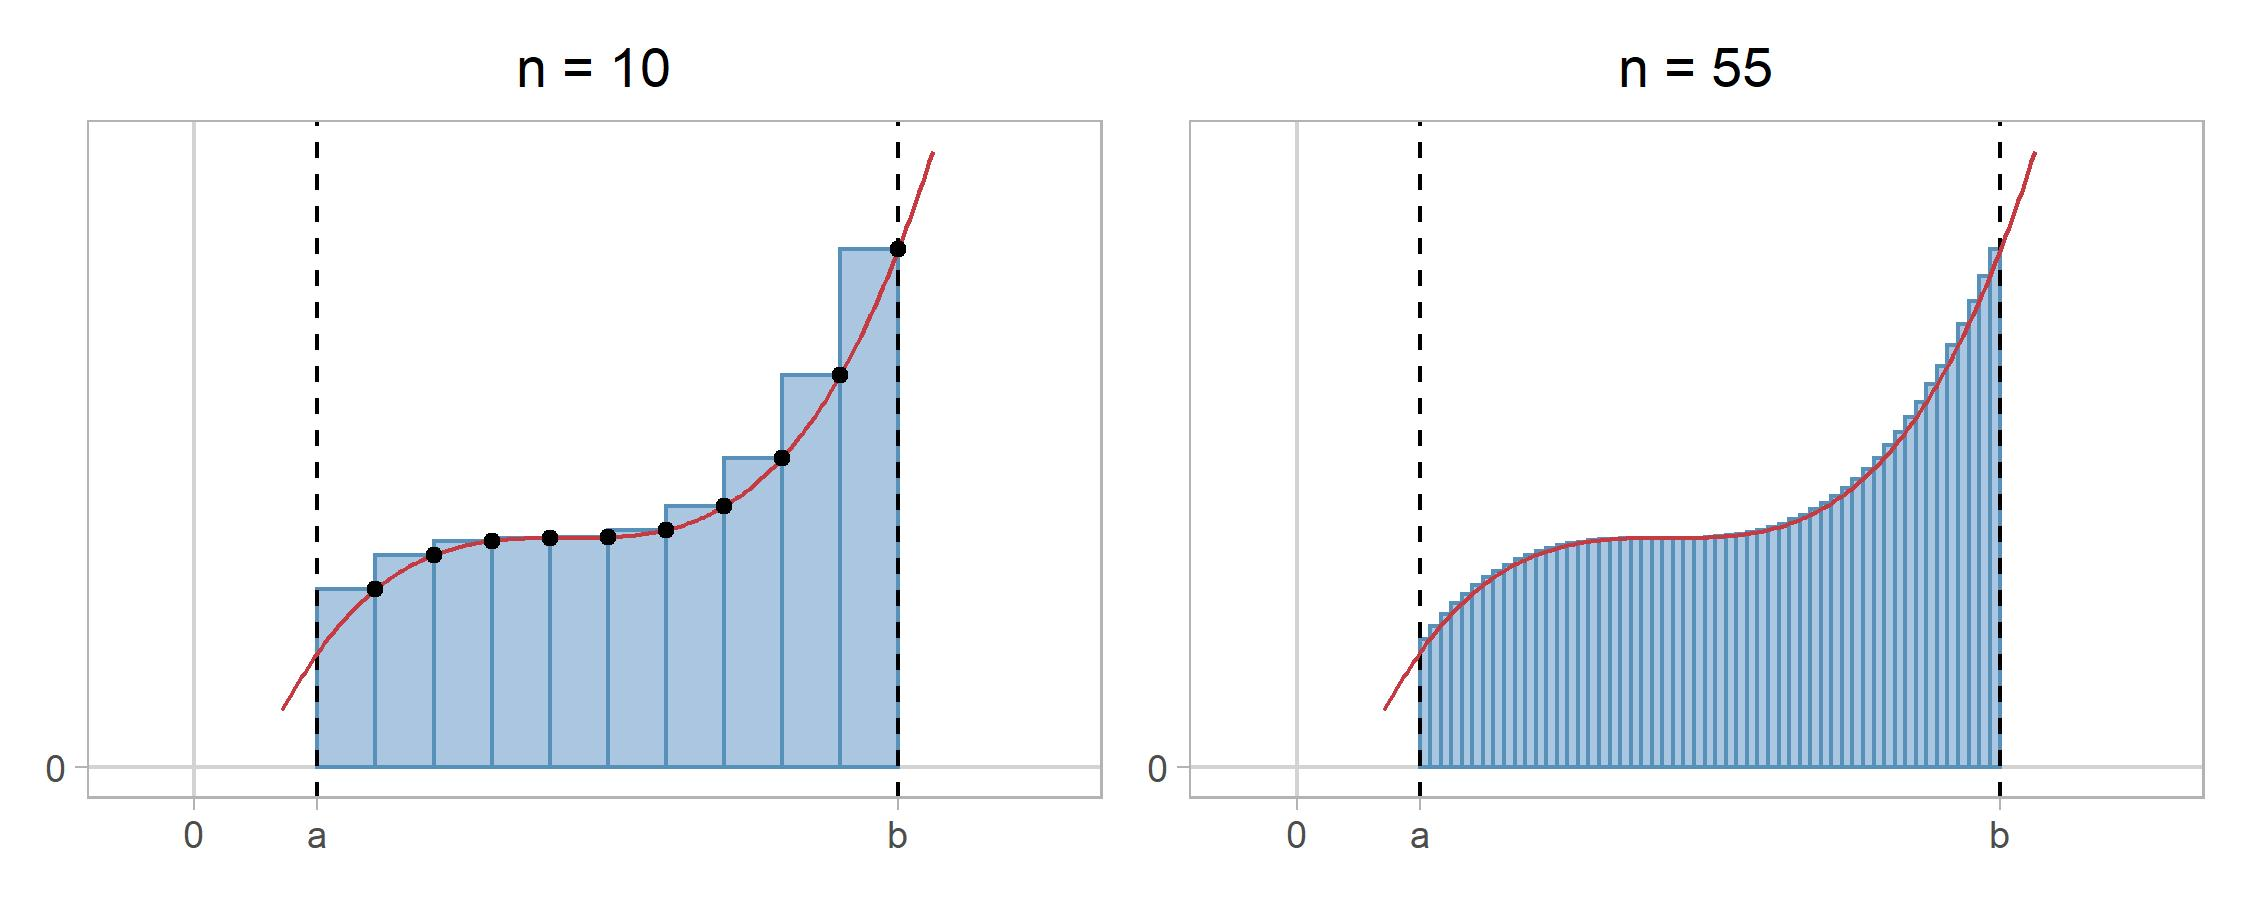
\includegraphics[scale=0.7]{img/area-under-curve-3.jpg}
\end{figure}

El problema es que, eventualmente, las bases y áreas de los rectángulos se igualarán a cero. Por lo tanto, en vez de buscar el valor exacto de la suma de Riemann, desde el Cálculo vemos a qué valor ésta converge a medida que $n$ se acerca al infinito, por medio de su límite.

Es por ello que la integral definida se la define como el \textbf{límite al infinito de la suma de Riemann}.

\subsection{El límite de la Suma de Riemann.}

Debido a que el área bajo la curva siempre lo dividimos en rectángulos de igual base, dicha medida podemos generalizarla como:
\[
  \Delta x = \frac{b - a}{n}
\]
Si tomamos un punto $(c_{i}, \ f(c_{i}))$, $\forall c_{i} \in [a, \ b]$, entre cada $\Delta x$ y $f(c_{i})$ se forman $n$ rectángulos de áreas $A = f(c_{i}) \cdot \Delta x$, donde $f(c_{i})$ es su altura y $\Delta x$ su base.

\begin{figure}[hbt!]
\centering
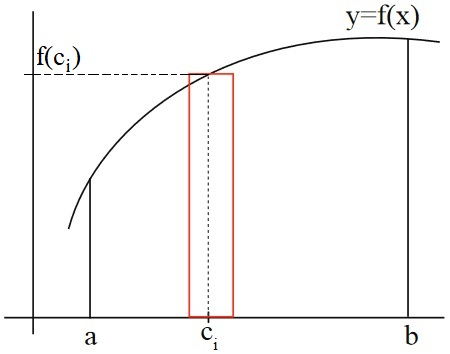
\includegraphics[scale=0.45]{img/riemann-sum.jpg}
\end{figure}

La suma de las áreas de los rectángulos desde $i = 1$ hasta $i = n$ corresponde a la \textbf{Suma de Riemann}.
\[
  \sum_{i = 1}^{n} f(c_{i}) \Delta x
\]
Si llevamos $n \to \infty$, obtenemos la \textbf{integral definida}:
\[
  \int_{a}^{b} f(x)dx = \lim_{n \to \infty} \left(\sum_{i = 1}^{n} f(c_{i}) \Delta x\right)
\]
Veamos que, a medida que $n \to \infty$, $\Delta x \to 0$. También, que $\Delta x$ se relaciona con $dx$ (diferencial de Leibniz), puesto que el primero refleja un incremento y el segundo igual, pero infinitesimal.

\textbf{Ejemplo 1.} \quad Calcule la $\int_{0}^{b} x^{2} dx$, con $b$ constante y $b > 0$, usando la suma de Riemann.

\newpage

\begin{figure}[hbt!]
\centering
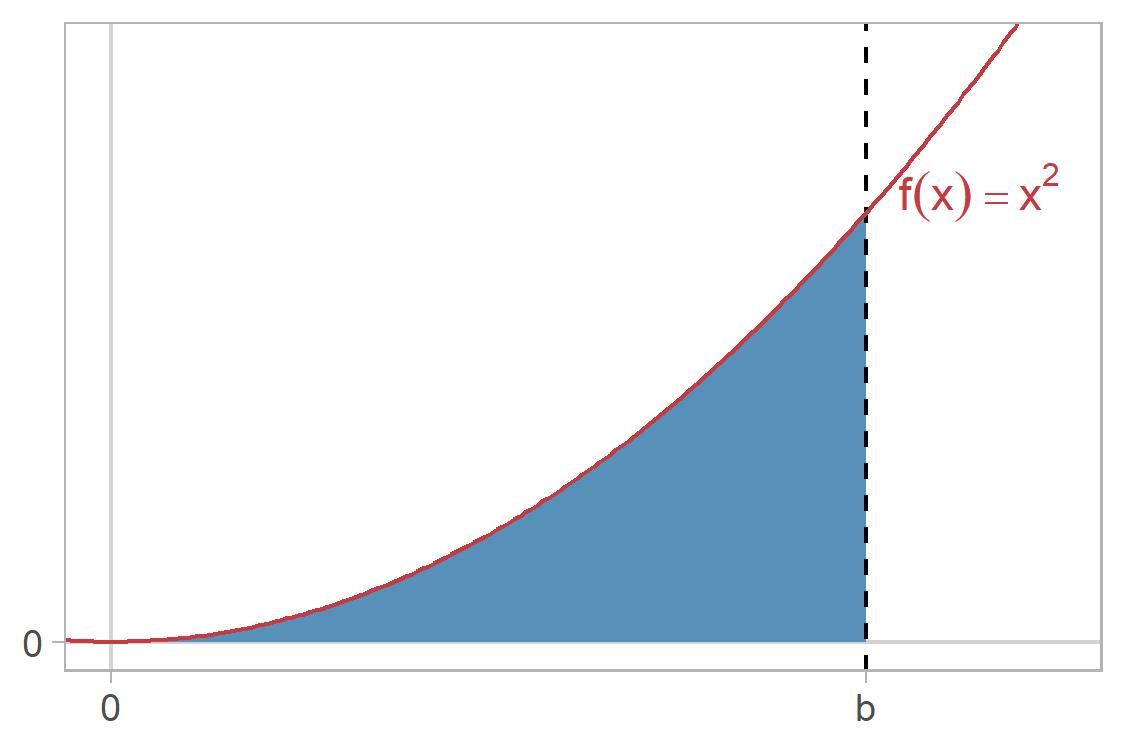
\includegraphics[scale = 0.7]{img/riemann_example-1.jpg}
\end{figure}

\textbf{Solución.} \quad Primero dividamos el área en $n$ rectángulos, cuyas longitudes de bases serán:
\[
  \Delta x = \frac{b - 0}{n} = \frac{b}{n}
\]
Luego, elijamos un valor $x = c_{i}$ para conocer la altura de cada rectángulo. En esta ocasión tomemos sus esquinas derechas, lo que implica que el primer valor será $c_{1} = b/n$. Por lo tanto, su altura será $f(c_{1}) = (b/n)^{2}$. A continuación tenemos un resumen de los $n$ puntos:

\begin{table}[hbt!]
\centering
\begin{tabular}{c|c c c c c c}
$i$ & $1$ & $2$ & $3$ & $\cdots$ & $n - 1$ & $n$ \\
\hline
$c_{i}$ & $b/n$ & $2b/n$ & $3b/n$ & $\cdots$ & $(n-1)b/n$ & $nb/n$ \\
\hline
$f(c_{i}) = (c_{i})^{2}$ & $(b/n)^{2}$ & $(2b/n)^{2}$ & $(3b/n)^{2}$ & $\cdots$ & $((n-1)b/n)^{2}$ & $(nb/n)^{2}$ 
\end{tabular}
\end{table}

En consecuencia, el área $A$ será la suma de las áreas de los $n$ rectángulos:
\[
  A = \left[\left(\frac{b}{n}\right)^{2} \cdot \frac{b}{n}\right] +
      \left[\left(\frac{2b}{n}\right)^{2} \cdot \frac{b}{n}\right] +
      \left[\left(\frac{3b}{n}\right)^{2} \cdot \frac{b}{n}\right] + \cdots +
      \left[\left(\frac{(n-1)b}{n}\right)^{2} \cdot \frac{b}{n}\right] +
      \left[\left(\frac{nb}{n}\right)^{2} \cdot \frac{b}{n}\right] 
\]

La cual podemos reducir como la siguiente suma de Riemann:
\[
  A = \sum_{i = 1}^{n} \left(\frac{i \cdot b}{n}\right)^{2} \cdot \frac{b}{n}
    = \sum_{i = 1}^{n} \left(\frac{b}{n}\right)^{3} \cdot i^{2}
\]
Debido a que $b$ y $n$ son constantes, podemos denotar esta suma como:
\[
  A = \left(\frac{b}{n}\right)^{3} \cdot \sum_{i = 1}^{n} i^{2}
\]
Posteriormente, tomamos el límite de esta suma para ver a qué valor converge a medida que $n \to \infty$.
\[
  \int_{0}^{b} x^{2} dx = \lim_{n \to \infty} A
                        = \lim_{n \to \infty} \left(\left(\frac{b}{n}\right)^{3} \cdot \sum_{i = 1}^{n} i^{2}\right)
\]
En el caso del límite, solo $b$ es constante. Por lo tanto:
\[
  \int_{0}^{b} x^{2} dx = b^{3} \cdot \lim_{n \to \infty} \left(\frac{1}{n^{3}} \cdot \sum_{i = 1}^{n} i^{2}\right)
\]
Para resolver el límite, usaremos una intuición geométrica en vez de algebraica\footnote{La intuición algebraica es más corta de la que veremos a continuación, porque se cumple que:\[\sum_{i = 1}^{n} i^{2} = \frac{n(n+1)(2n+1)}{6}\]Por lo tanto, solo tendríamos que reemplazar aquella expresión en el límite para encontrar el valor de la integral definida. No obstante, la intuición geométrica no deja de ser interesante.}, basándonos en el volúmen de una pirámide escalonada, con cada base de lado $i$ y de alturas iguales a $1$.

\begin{figure}[hbt!]
\centering
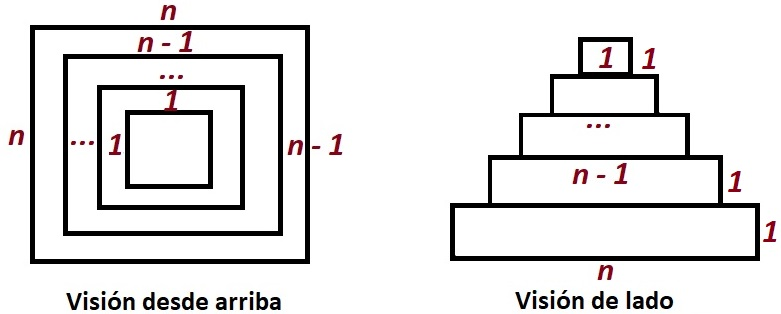
\includegraphics[scale=0.4]{img/riemann-pyramid.jpg}
\end{figure}

Cada bloque de la pirámide es un prisma cuadrado, cuyo volumen es el producto entre el área de su base $i^{2}$ y su altura $1$. Si los sumamos\footnote{Como una suma de Riemann.}, podemos obtener el volumen de la pirámide escalonada, $V_{T}$.
\[
  V_{T} = (1^{2} \cdot 1) + (2^{2} \cdot 1) + \cdots + (n^{2} \cdot 1)
        = \sum_{i = 1}^{n} (i^{2} \cdot 1)
        = \sum_{i = 1}^{n} i^{2}
\]
Para estimar esta suma, vamos a trazar pirámides lisas adentro y afuera de la escalonada, donde las aristas (bordes) de las primeras tienen una pendiente de $\pm 2$ y las segundas son paralelas a estas últimas. Por otra parte, sus alturas son $n$ y $n + 1$, respectivamente.

\begin{figure}[hbt!]
\centering
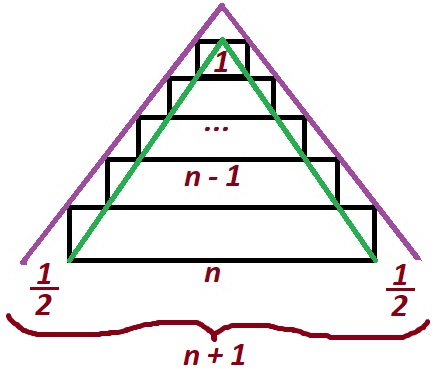
\includegraphics[scale=0.4]{img/riemann-pyramid-2.jpg}
\end{figure}

El volumen de una pirámide lisa corresponde a $1/3$ del producto entre el área de su base y su altura. Por lo tanto, sea $V_{Int}$ el volumen de la pirámide de adentro y $V_{Ext}$ de la que está afuera, podemos establecer a partir de la imagen de arriba que:
\begin{align*}
  V_{Int} &< V_{T} < V_{Ext} \\
  \frac{1}{3} n^{2} \cdot n &< \sum_{i = 1}^{n} i^{2} < \frac{1}{3} (n + 1)^{2} \cdot (n + 1) \\
  \frac{1}{3} n^{3} &< \sum_{i = 1}^{n} i^{2} < \frac{1}{3} (n + 1)^{3}
\end{align*}
Recordemos que nuestro propósito es conocer el valor del límite en $\int_{0}^{b} x^{2} dx$ por medio de $V_{T}$. Por lo tanto, multipliquemos por $1/n^{3}$ a la desigualdad de arriba.
\begin{align*}
  \frac{1}{3} \cdot \left(\frac{n^{3}}{n^{3}}\right) &<
  \frac{1}{n^{3}} \cdot \sum_{i = 1}^{n} i^{2} <
  \frac{1}{3} \frac{(n + 1)^{3}}{n^{3}} \\
  \frac{1}{3} &<
  \frac{1}{n^{3}} \cdot \sum_{i = 1}^{n} i^{2} <
  \frac{1}{3} \left(1 + \frac{1}{n}\right)^{3}
\end{align*}

Finalmente, para estimar el volumen de la pirámide escalonada, tomemos el límite en la desigualdad a medida que $n \to \infty$.
\begin{align*}
  \lim_{n \to \infty} \frac{1}{3} &<
  \lim_{n \to \infty} \left(\frac{1}{n^{3}} \cdot \sum_{i = 1}^{n} i^{2}\right) <
  \lim_{n \to \infty} \left[\frac{1}{3} \left(1 + \frac{1}{n}\right)^{3}\right] \\
  \frac{1}{3} &<
  \lim_{n \to \infty} \left(\frac{1}{n^{3}} \cdot \sum_{i = 1}^{n} i^{2}\right) <
  \frac{1}{3}
\end{align*}
En otras palabras:
\[
  \lim_{n \to \infty} \left(\frac{1}{n^{3}} \cdot \sum_{i = 1}^{n} i^{2}\right) = \frac{1}{3}
\]
Por consiguiente:
\[
  \int_{0}^{b} x^{2} dx = b^{3} \cdot \frac{1}{3} = \frac{b^{3}}{3}
\]

\subsubsection{Detectando un patrón.}

Veamos el siguiente caso.

\textbf{Ejemplo 2.} \quad Calcule (a) $\int_{0}^{b} x dx$ y (b) $\int_{0}^{b} 1 dx$, con $b > 0$.

\newpage

\begin{figure}[hbt!]
\centering
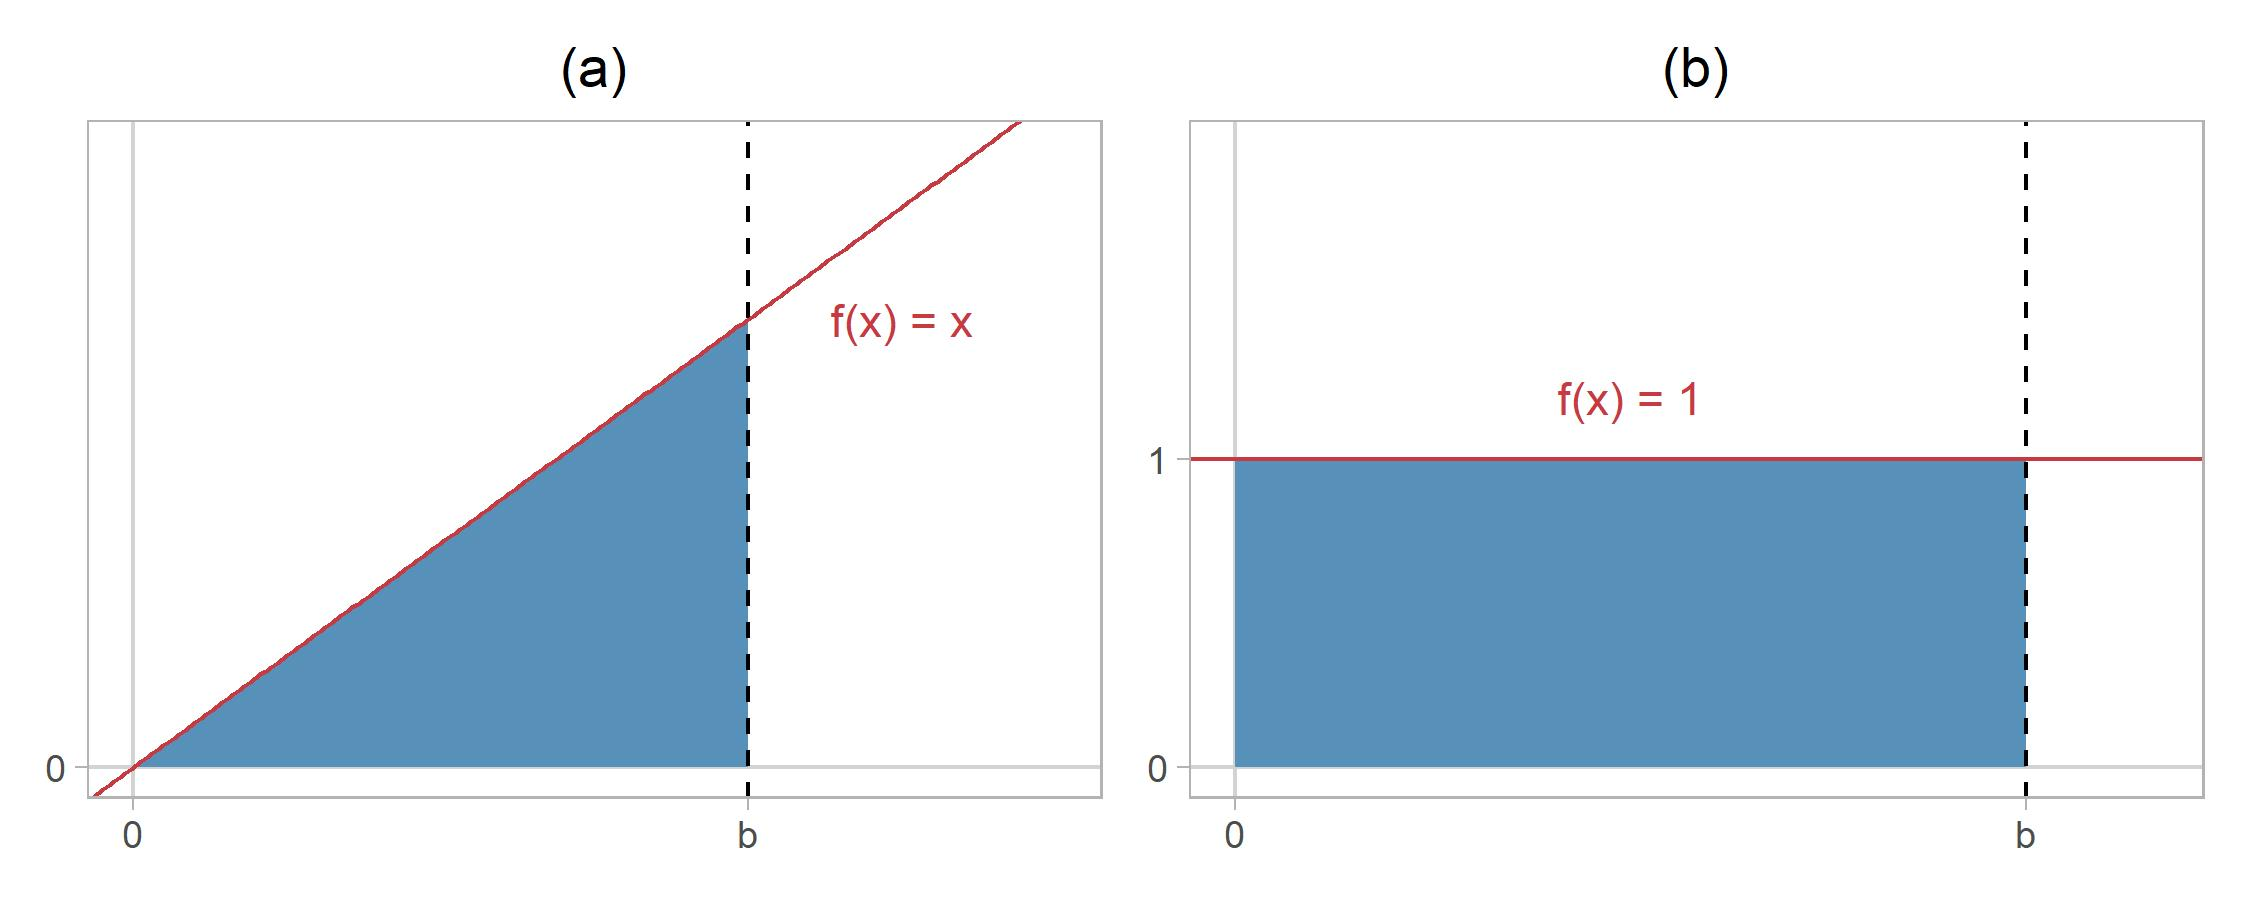
\includegraphics[scale = 0.7]{img/riemann_example-2.jpg}
\end{figure}

\textbf{Solución.} \quad La integral (a) corresponde al área del triángulo (en este caso, rectángulo):
\[
  \int_{0}^{b} x dx = \frac{1}{2} b \cdot b = \frac{1}{2} b^{2}
\]
Mientras que la superficie bajo la curva de (b) es el área de un rectángulo:
\[
  \int_{0}^{b} 1 dx = b \cdot 1 = b
\]
Si consideramos, el ejercicio anterior y mantenemos que $b > 0$, es posible observar el siguiente patrón:

\begin{table}[hbt!]
\centering

\begin{tabular}{c|c c c}
$f(x)$ & $x^{0} = 1$ & $x^{1} = x$ & $x^{2}$ \\
\hline
$\int_{0}^{b} f(x) dx$ & $b = b^{1}/1$ & $b^{2}/2$ & $b^{3}/3$
\end{tabular}

\end{table}

Por lo tanto, es válido suponer que $\int_{0}^{b} x^{3}dx = b^{4}/4$. De manera que podemos generalizar este patrón como:
\[
  \int_{0}^{b} x^{k} dx = \frac{b^{k + 1}}{k + 1} \quad (k \neq -1, \ a = 0 \text{ y } b > a)
\]


\subsection{La Integral Definida como una Suma Acumulada.}

Hasta ahora hemos estudiado a la integral definida como el área bajo una curva. Ésta es su explicación geométrica, pero en términos generales, corresponde a una \textbf{Suma Acumulada}.

\textbf{Ejemplo 3.} \quad Supongamos que tenemos la idea de pedir préstamos a un banco y queremos modelar tanto el dinero recibido cada año asumiendo que lo hacemos todos los días, como la deuda con la que quedaremos.

Para modelar el dinero total, establezcamos que $t$ es una variable de tiempo en años y $f(t)$ es la tasa de préstamo (\textit{borrowing rate}) medido en \$ por año. Además, como asumimos que pedimos dinero todos los días, multipliquemos esta función por $\Delta t = 1/365$ también medido en años, para hacer el seguimiento del dinero prestado en cada incremento de tiempo (i.e, en cada día).

En ese sentido, para medir cuánto dinero pedimos prestado ($P$) el día $45$ de un año (i.e, en $t = 45/365$), calculamos:
\[
  P = f\left(\frac{45}{365}\right) \left(\frac{\$}{\text{años}}\right) \cdot \frac{1}{365} (\text{años})
    = f\left(\frac{45}{365}\right) \cdot \Delta t \ (\$)
\]
Por lo tanto, el dinero prestado total en cada año ($P_{T}$) será la suma de aquellos préstamos diarios:
\[
  P_{T} = \left(\sum_{i = 1}^{365} f\left(\frac{i}{365}\right) \cdot \Delta t \right) \ (\$)
\]
Si observamos bien, la cantidad de sumas que debemos calcular para saber cuánto dinero pediríamos prestado en más de un año, sería enorme (no olvidemos que es en cada día). Por lo tanto es válido asumir que $P_{T}$ será muy similar a la siguiente integral:
\[
  P_{T} = \left(\sum_{i = 1}^{365} f\left(\frac{i}{365}\right) \cdot \Delta t\right) \ (\$)
         \sim \int_{0}^{1} (f(t) dt) \ (\$)
\]
Si bien es posible hacer un seguimiento de la sumatoria, es mucho más óptimo hacerlo con una integral en términos de tiempo, por ejemplo.

Ahora necesitamos modelar la deuda con la que quedaremos en cada año por el dinero prestado. Para ello, usaremos un \href{https://en.wikipedia.org/wiki/Compound_interest#Continuous_compounding}{interés compuesto continuo} \footnote{Se escribe más genéricamente como $C_{t} = C_{0} \cdot \exp(it)$, con $C_{t}$ siendo el capital final y $C_{0}$ el capital inicial.}, donde $D$ es la deuda (i.e, el capital final), $P$ es el dinero prestado en un año (i.e, capital inicial), $i$ es una tasa de interés anual y $t$ el tiempo en años:
\[
  D = P \cdot \exp(it)
\]
La deuda total $D_{T}$ de las veces que pedimos prestado dinero será las sumas de cada deuda $D$, donde $i$ será multiplicado a la cantidad de tiempo que queda en un año, $t = 1 - (i/365)$ años.
\[
D_{T} = \sum_{i = 1}^{365} P \cdot \exp(it)
      = \sum_{i = 1}^{365} \left[f\left(\frac{i}{365}\right) \cdot \Delta t \right] \cdot
        \exp\left[i \cdot \left(1 - \frac{i}{365}\right)\right]
\]

\newpage

Al igual que con el dinero total prestado, la deuda total también irá convergiendo a la siguiente integral definida por el mismo motivo:
\[
  D_{T} = \sum_{i = 1}^{365} \left[f\left(\frac{i}{365}\right) \cdot \Delta t \right] \cdot
          \exp\left[i \cdot \left(1 - \frac{i}{365}\right)\right]
        \sim \int_{0}^{1} \exp(i \cdot (1 - t)) \cdot f(t)dt
\]
Veamos que, en síntesis, tanto el dinero total prestado como la deuda total fueron \textbf{Sumas acumuladas}, las que correspondieron a \textbf{integrales definidas}.





\end{document}
